% !Mode:: "TeX:UTF-8"
\documentclass[xcolor=svgnames,serif,table,10pt]{beamer}
%\includeonlyframes{Representation}%Acknowledgement
\mode<presentation>{
% Setup appearance:
\setbeamercovered{transparent}
\usecolortheme[named=FireBrick]{structure}
\setbeamertemplate{caption}[numbered]
\setbeamertemplate{navigation symbols}{}

\useoutertheme{infolines}
\usetheme{Darmstadt}

\setbeamertemplate{blocks}[rounded][shadow=true]
\setbeamercovered{transparent}

% 修改样式
%\setbeamertemplate{blocks}[rounded][shadow=true]

\setbeamercolor{box}{bg=black!20!orange,fg=white}

\setbeamercolor{block title}{use=sidebar,fg=sidebar.fg!10!white,bg=orange!70!black}
%\setbeamercolor{block body}{use=sidebar,fg=black,bg=sidebar.bg!90!blue}

\setbeamercolor{block title example}{use=sidebar,fg=sidebar.fg!10!white,bg=black!60!green}
%\setbeamercolor{block body example}{use=sidebar,fg=black,bg=sidebar.bg!90!green}

\setbeamercolor{block title alerted}{use=sidebar,fg=sidebar.fg!10!white,bg=black!50!red}
%\setbeamercolor{block body alerted}{use=sidebar,fg=black,bg=sidebar.bg!90!red}

\setbeamerfont{frametitle}{size=\small,series=\CJKfamily{FZDH}\Arial\boldmath}
%\setbeamerfont{frametitle}{series=\bfseries}

\setbeamertemplate{headline}
{%
  \begin{beamercolorbox}[shadow=true]{section in head/foot}
  \vskip2pt\insertnavigation{\paperwidth}\vskip2pt
  \end{beamercolorbox}%
}

\iffalse
\AtBeginSection[]
{
  \frame{
    \footnotesize
    \frametitle{主要内容}
    \tableofcontents[currentsection]
  }
}

\AtBeginSubsection[]
{
  \begin{frame}
    \footnotesize
    \frametitle{主要内容}
    \tableofcontents[currentsection,currentsubsection]
  \end{frame}
}
\fi

\renewcommand{\raggedright}{\leftskip=0pt \rightskip=0pt plus 0cm}
\raggedright
}

\usepackage{tabularx,multirow,multicol,longtable}
\usepackage{tabu}
\usepackage{graphics}
\usepackage{xcolor}
\usepackage[no-math]{fontspec}%--------------------------------------------------提供字体选择命令
\usepackage{xunicode}%-----------------------------------------------------------提供Unicode字符宏
\usepackage{xltxtra}%------------------------------------------------------------提供了针对XeTeX的改进并且加入了XeTeX的LOGO
\usepackage[BoldFont,SlantFont,CJKchecksingle]{xeCJK}%---------------------------使用xeCJK宏包
%================================== 设置中文字体 ================================%
\setCJKmainfont[BoldFont={SimHei},ItalicFont={KaiTi}]
  {SimSun}
\setCJKsansfont{SimHei}
\setCJKmonofont{[SIMFANG.TTF]}

\setCJKfamilyfont{zhsong}{SimSun}
\setCJKfamilyfont{zhhei}{SimHei}
\setCJKfamilyfont{zhkai}{KaiTi}
\setCJKfamilyfont{zhfs}{FangSong}
\setCJKfamilyfont{zhli}{LiSu}
\setCJKfamilyfont{zhyou}{YouYuan}

\newcommand*{\songti}{\CJKfamily{zhsong}} % 宋体
\newcommand*{\heiti}{\CJKfamily{zhhei}}   % 黑体
\newcommand*{\kaishu}{\CJKfamily{zhkai}}  % 楷书
\newcommand*{\fangsong}{\CJKfamily{zhfs}} % 仿宋
\newcommand*{\lishu}{\CJKfamily{zhli}}    % 隶书
\newcommand*{\youyuan}{\CJKfamily{zhyou}} % 幼圆
%================================== 设置中文字体 ================================%

%================================== 设置英文字体 ================================%
\setmainfont[Mapping=tex-text]{TeX Gyre Pagella}%--------------------------------英文衬线字体
\setsansfont[Mapping=tex-text]{Trebuchet MS}%------------------------------------英文无衬线字体
\setmonofont[Mapping=tex-text]{Courier New}%-------------------------------------英文等宽字体
\newfontfamily\Arial{Arial}
%================================== 设置英文字体 ================================%

%================================== 设置数学字体 ================================%
%\setmathsfont(Digits,Latin,Greek)[Numbers={Lining,Proportional}]{Minion Pro}
%================================== 设置数学字体 ================================%
\punctstyle{kaiming}%------------------------------------------------------------开明式标点格式
\usepackage{graphicx}
\usepackage{tikz}
\usetikzlibrary{positioning,backgrounds}
\usetikzlibrary{fadings}
\usetikzlibrary{patterns}
\usetikzlibrary{calc}
\usetikzlibrary{shadings}
\pgfdeclarelayer{background}
\pgfdeclarelayer{foreground}
\pgfsetlayers{background,main,foreground}
\usepackage{xifthen}
\usepackage{colortbl,dcolumn}
\usepackage{enumerate}
\usepackage{pifont}
\usepackage{tabularx}
\usepackage{booktabs}

%=================================== 数学符号 =================================%
\newcommand{\rtn}{\mathrm{\mathbf{R}}}
\newcommand{\N}{\mathrm{\mathbf{N}}}
\newcommand{\As}{\mathrm{a.s.}}
\newcommand{\Ae}{\mathrm{a.e.}}
\newcommand*{\PR}{\mathrm{\mathbf{P}}}
\newcommand*{\EX}{\mathrm{\mathbf{E}}}
\newcommand{\EXlr}[1]{\mathrm{\mathbf{E}}\left[#1\right]}
\newcommand*{\dif}{\,\mathrm{d}}
\newcommand*{\F}{\mathcal{F}}
\newcommand*{\h}{\mathcal{H}}
\newcommand*{\vp}{\varepsilon}
\newcommand*{\prs}{\dif\PR-\As}
\newcommand*{\dte}{\dif t-\Ae}
\newcommand*{\pts}{\dif\PR\times\dif t-\Ae}
\newcommand{\Ito}{It\^{o}}
\newcommand{\tT}[1][0]{[#1,T]}
\newcommand{\intT}[2][T]{\int^{#1}_{#2}}
\newcommand{\intTe}[1][t]{\intT[t+\varepsilon]{#1}}
\newcommand{\s}{\mathcal{S}}
\newcommand{\me}{\mathrm{e}}
\newcommand{\one}[1]{{\bf 1}_{#1}}
\renewcommand{\M}{{\rm M}}
\newcommand{\Me}[1][t]{M^{\varepsilon}_{#1}}
\newcommand{\Ne}[1][t]{N^{\varepsilon}_{#1}}
\newcommand{\Pe}[1][t]{P^{\varepsilon}_{#1}}
\DeclareMathOperator*{\sgn}{sgn}
%=================================== 数学符号 =================================%

\graphicspath{{figures/}}

\title[2010 级硕士学位答辩 (BSDE)]{一类倒向随机微分方程 \boldmath$L^p$ $(p\geq 1)$ 解的\\ 存在惟一性及生成元的表示定理}

\author[肖立顺]
{姓名: \makebox[4em][s]{肖立顺}\\
  导师: \makebox[4em][s]{范胜君}\\
  专业: \makebox[4em][s]{应用数学}\\
  方向: \makebox[4em][s]{随机分析}}

\institute[CUMT]{
\includegraphics[width=1cm]{cumt.pdf}\\ 2010 级硕士学位论文答辩}

\date{\tiny 2013-05-21}

\setlength{\baselineskip}{22pt}
\renewcommand{\baselinestretch}{1.4}

\begin{document}

\setlength{\abovedisplayskip}{1ex}%------------------------------------------ 公式前的距离
\setlength{\belowdisplayskip}{1ex}%------------------------------------------ 公式后的距离

%\includeonlyframes{Brown}

\begin{frame}
  \titlepage
\end{frame}

\begin{frame}{内容提纲}
\begin{figure}
\vskip-2.5em
  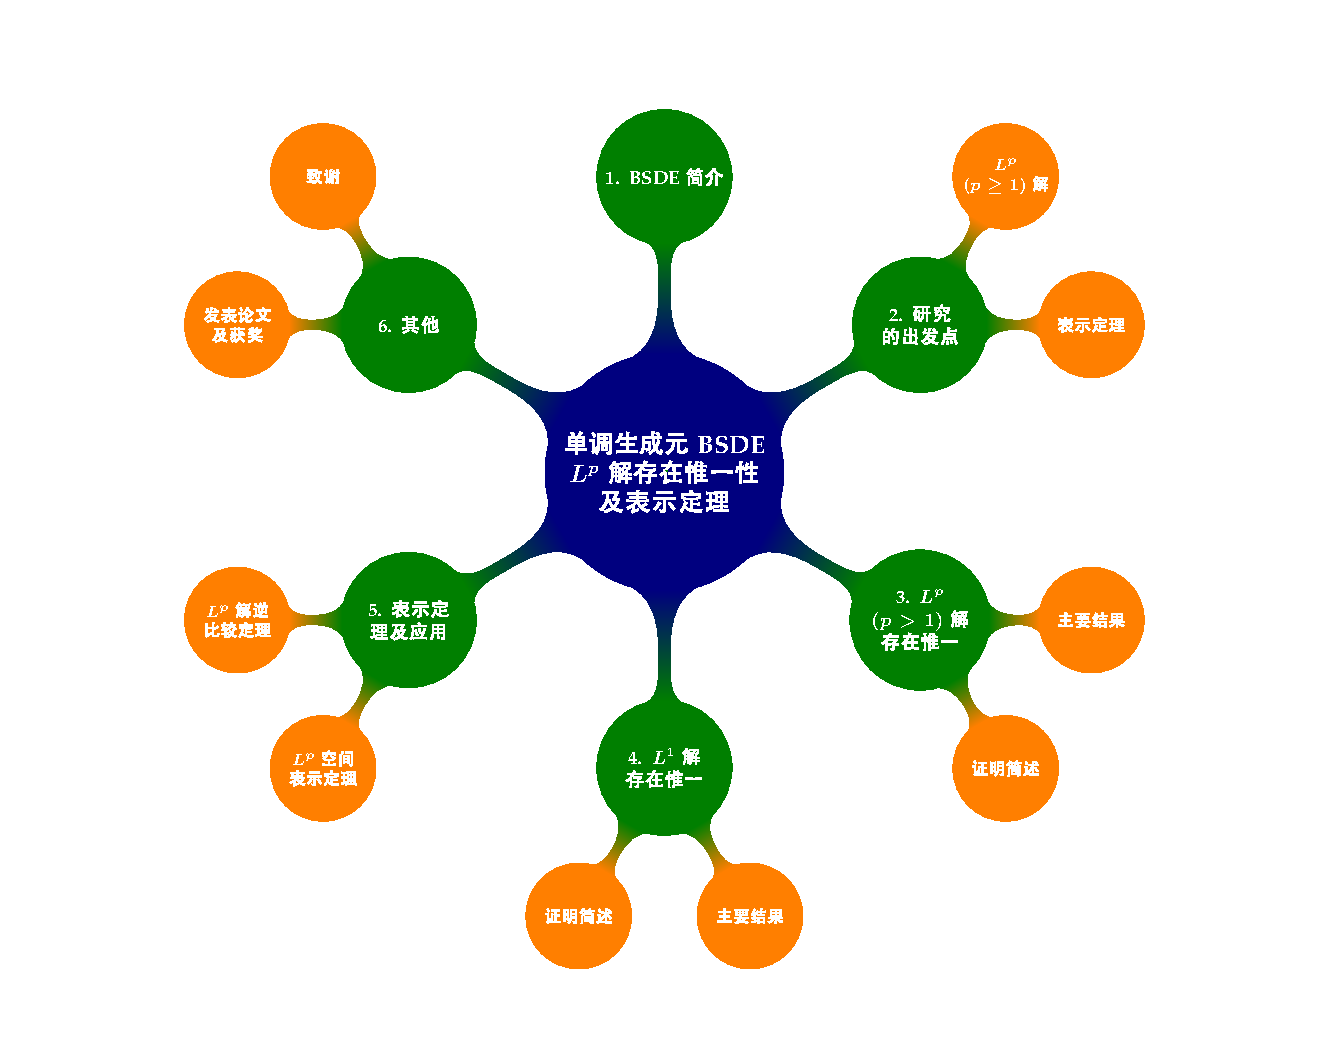
\includegraphics[page=1,scale=0.5]{mainmap}
\end{figure}
\end{frame}

\section{BSDE 简介}
\begin{frame}{倒向随机微分方程 (BSDE) 简介}
\begin{figure}
\vskip-2.5em
  \includegraphics[page=2,scale=0.5]{mainmap}
\end{figure}
\end{frame}

\begin{frame}[t]{倒向随机微分方程 (BSDE) 简介}

\qquad 线性的倒向随机微分方程 (BSDE) 由 \cite{Bismut1973JMAA} 提出;

\qquad \cite{PardouxPeng1990SCL} 提出非线性 BSDE 如下:

\medskip
  \begin{beamercolorbox}[shadow=true,sep=0pt,rounded=true]{box}
    \begin{equation}\label{eq:BSDEs}
      {\color<6>[rgb]{0,0,0}y_t}={\color<3,5>[rgb]{0,0,0}\xi}+
          \int_t^{{\color<2,5>[rgb]{0,0,0}T}} {\color<4,5>[rgb]{0,0,0}g}(s,{\color<6>[rgb]{0,0,0}y_s},{\color<6>[rgb]{0,0,0}z_s})\dif s
          -\int_t^{{\color<2,5>[rgb]{0,0,0}T}}{{\color<6>[rgb]{0,0,0}z_s}\dif B_s},\quad t\in[0,{\color<2,5>[rgb]{0,0,0}T}].
    \end{equation}
  \end{beamercolorbox}

\pause

 \begin{center}
  \setlength{\extrarowheight}{1.5mm}
  %\addtolength{\tabcolsep}{1mm}
  \rowcolors[]{1}{orange!70}{white!90!gray}
   \begin{tabular}{cl}
      \onslide<2->{$T$}         & \onslide<2->{终端时间, $0\leq T\leq +\infty$} \\
      \onslide<3->{$\xi$}       & \onslide<3->{终端条件, 可测随机变量}\\
      \onslide<4->{$g$}         & \onslide<4->{生成元, $g(\omega,t,y,z):\Omega\times[0,T]\times\rtn^k\times\rtn^{k\times d}\to\rtn^k$}\\
      \onslide<5->{$(\xi,T,g)$} & \onslide<5->{BSDE 的参数}\\
      \onslide<6->{$(y_t,z_t)_{t\in\tT}$} & \onslide<6->{BSDE 的适应解}\\
    \end{tabular}
 \end{center}
\end{frame}

\begin{frame}{倒向随机微分方程 (BSDE) 简介}
  \begin{itemize}
    \item \cite{DuffieEpstein1992Econometrica}, \alert{效用函数理论};
    \item \mbox{[Peng(1991)]}, \alert{反应扩散方程}和 \alert{Navier-Stokes 方程};
    \item \cite{ElKarouiPengQuenez1997MF}, \alert{派生证券} (如期权期货等);
    \item \mbox{[Peng(1997)]}, $g$-期望和条件 $g$-期望, \alert{金融风险度量};
    \item 反射倒向随机微分方程 (RBSDE), 正倒向随机微分方程 (FBSDE), 倒向重随机微分
          方程 (BDSDE), 以及带跳的、超前的 BSDE;
    \item 解的性质: [Peng(1992)] 提出 BSDE 解的比较定理;
    \item \cite{BriandCoquetHuMeminPeng2000ECIP} 提出解的逆比较定理, 生成元表示定理;
    \item \ldots\ldots \ \ldots\ldots
  \end{itemize}
\end{frame}

\begin{frame}{倒向随机微分方程 (BSDE) 简介}
\scriptsize
  \begin{block}{$(Y_t)_{t\in\tT}$ 所在的空间}
    ${\s}^p(0,T;\rtn^k)$  表示 $\rtn^k$-值, 适应且满足
    $$\|Y\|_{{\s}^p}:=
    \left(\EX
      \left[
        \sup_{t\in\tT}|Y_t|^p
      \right]
    \right)^{1\wedge 1/p}<+\infty$$
    的连续过程 $(Y_t)_{t\in\tT}$ 全体.
  \end{block}

  \begin{block}{$(Z_t)_{t\in\tT}$ 所在的空间}
    $\M^p(0,T;\rtn^{k\times d})$ 表示
    ${\rtn}^{k\times d}$-值, $(\F_t)$-循序可测且满足
    $$\|Z\|_{{\M}^p}:=
      \left\{\EX
      \left[
        \left(
          \int_0^T |Z_t|^2\dif t
        \right)^{p\over 2}
      \right]
      \right\}^{1\wedge 1/p}<+\infty$$
    的连续过程 $(Z_t)_{t\in\tT}$ 全体.
  \end{block}

  \qquad 连续过程 $(Y_t)_{t\in\tT}$ 属于 (D) 类是指, 随机过程族
$\{Y_\tau:\tau\in\Sigma_T\}$
是一致可积的, 其中 $\Sigma_T$ 表示所有满足 $\tau\leq T$ 的停时全体.
\end{frame}

\section{研究的出发点}

\begin{frame}{研究的出发点}
\begin{figure}
\vskip-2.5em
  \includegraphics[page=3,scale=0.5]{mainmap}
\end{figure}
\end{frame}

\subsection{$L^p$ $(p\geq 1)$ 解的存在惟一性}

\begin{frame}[label=LpExistence]{$L^p$ $(p\geq 1)$ 解的存在惟一性}
\vspace{-2ex}
\def\xslant{-0.6}
\def\yslant{0.5}
\tiny
\tikzstyle{circleL2}=[ball color=red!80!black,circle,anchor=base,scale=1]
\tikzstyle{circleLp}=[ball color=green!80!black,circle,anchor=base,scale=1]
\tikzstyle{circleInfinity}=[ball color=orange!80!black,circle,anchor=base,scale=1]
\tikzstyle{circleL1}=[ball color=teal!80,circle,anchor=base,scale=1]
\tikzstyle{ToTeal}=[->,>=stealth,shorten <=0pt,shorten >=0pt,semithick,teal!80!black]
%\tikzstyle{ToBlue}=[->,>=stealth,shorten <=0pt,shorten >=0pt,semithick,blue!80!black]
\tikzstyle{ToOrange}=[->,>=stealth,shorten <=0pt,shorten >=0pt,semithick,orange!50!red]
\begin{tikzpicture}[scale=.6,every node/.style={minimum size=1mm}]
  %-------------layer of L2
  \begin{scope}[
	yshift=-120,rounded corners=5pt,
	every node/.append style={yslant=\yslant,xslant=\xslant},
	yslant=\yslant,xslant=\xslant]

    \visible<1->{
	\draw[red!50,dashed,thin,fill=red!20] (0,0) rectangle (6,5);

    \node[circleL2] (PP1990) at (0.36,4.0) {};
    \node[anchor=west] (PardouxPeng1990) at (0.5,4.0) {Pardoux-Peng [1990]};
    \node[anchor=west] (Lipschitz) at (1.5,3.5) {$g$ 关于 $(y,z)$ Lipschitz};
    }

    \visible<2->{
    \node[circleL2] (M1995) at (0.36,3.0) {};
    \node[anchor=west] (Mao1995) at (0.5,3.0) {Mao [1995]};
    \node[anchor=west] (MaoCondition) at (2.5,3.0) {Mao 氏条件};
    \draw[ToTeal] (PP1990) to[out=-90,in=90] (M1995);
    }

    \visible<3->{
    \node[circleL2] (LS1997) at (0.36,2.5) {};
    \node[anchor=west] (Lepeltier1997) at (0.5,2.5) {Lepeltier-San Martin [1997]};
    \node[anchor=west] (LinearGrowth) at (1.5,2.0) {$g$ 关于 $(y,z)$ 线性增长};
    \draw[ToTeal] (PP1990) to[out=-30,in=70] (LS1997);
    }

    \visible<4->{
    \node[circleL2] (P1999) at (0.36,1.5) {};
    \node[anchor=west] (Pardoux1999) at (0.5,1.5) {Pardoux [1999]};
    \node[anchor=west] (Monotonicity) at (2.56,1.5) {$g$ 关于 $y$ 单调且任意增长};
    \draw[ToTeal] (PP1990) to[out=-10,in=60] (P1999);
    }

    \visible<5->{
    \node[circleL2] (DotsL2) at (0.36,1) {};
    \node[anchor=west] at (0.5,1) {\ldots \ldots\ \ldots \ldots};
    }

    \visible<6->{
    \node[fill=white,rounded corners=0pt] at (3,0.5) {$L^2$ 解, $0\leq T<+\infty$};
    }
  \end{scope}
  %-------------layer of Lp
  \begin{scope}[
    yshift=-120,rounded corners=5pt,
    every node/.append style={yslant=\yslant,xslant=\xslant},
    yslant=\yslant,xslant=\xslant]

    \visible<7->{
    \fill[green!20,fill opacity=.70] (6.3,0) rectangle (12,5);
    \draw[green!80!black,dashed,thin] (6.3,0) rectangle (12,5);
    \node[fill=white,rounded corners=0pt] at (9.2,0.5) {$L^p$ 解, $0\leq T<+\infty$};
    }

    \visible<8->{
    \node[circleLp] (EP1997) at (6.66,4.0) {};
    \node[anchor=west] (ElKarouiPengQuenez1997) at (6.8,4.0) {El Karoui-Peng-Quenez [1997]};
    \node[anchor=west] (LipschitzP) at (7.3,3.5) {$g$ 关于 $(y,z)$ Lipschitz};
    \draw[ToTeal] (PP1990) to[out=40,in=150] (EP1997);
    }

    \visible<9->{
    \node[circleLp] (BC2000) at (6.66,3.0) {};
    \node[anchor=west] (BriandCarmona2000) at (6.8,3.0) {Briand-Carmona [2000]};
    \node[anchor=west] (PolynomialGrowth) at (7.3,2.5) {$g$ 关于 $y$ 单调且多项式增长};
    \draw[ToTeal] (EP1997) to[out=-90,in=90] (BC2000);
    }

    \visible<10->{
    \node[circleLp] (BD2003Lp) at (6.66,2.0) {};
    \node[anchor=west] (BriandDelyon2003Lp) at (6.8,2.0) {Briand-Delyon et al. [2003]};
    \node[anchor=west] (GeneralGrowthLp) at (7.3,1.5) {$g$ 关于 $y$ 单调且广义一般增长};
    \draw[ToTeal] (BC2000) to[out=-90,in=90] (BD2003Lp);
    }

    \visible<11->{
    \node[circleLp] (DotsLp) at (6.66,1.0) {};
    \node[anchor=west] at (6.8,1.0) {\ldots \ldots\ \ldots \ldots};
    }
  \end{scope}
  %-------------layer of L1
  \begin{scope}[
    yshift=0,rounded corners=5pt,
    every node/.append style={yslant=\yslant,xslant=\xslant},
    yslant=\yslant,xslant=\xslant]

    \visible<12->{
    \fill[teal!30,fill opacity=.70] (4.3,0.2) rectangle (10.2,6);
    \draw[teal, dashed, thin] (4.3,0.2) rectangle (10.2,6);
    \node[fill=white,rounded corners=0pt] at (7.2,0.9) {$L^1$ 解};
    }

    \visible<13->{
    \node[circleL1] (BD2003L1) at (4.66,5) {};
    \node[anchor=west] (BriandDelyon2003L1) at (4.8,5) {Briand-Delyon et al. [2003]};
    \node[anchor=west] (GeneralGrowthL1) at (5.3,4.5) {$g$ 关于 $y$ 单调且广义一般增长};
    \draw[ToTeal] (BD2003Lp) to[out=50,in=-30] (BD2003L1);
    }

    \visible<14->{
    \node[circleL1] (FL2010) at (4.66,4) {};
    \node[anchor=west] (FanLiu2010) at (4.8,4) {Fan-Liu [2010]};
    \node[anchor=west] (AlphaHolder) at (4.8,3.5) {关于 $y$ Lipschitz, 关于 $z$ $\alpha$-H\"older};
    }

    \visible<21->{
    \node[circleL1] (ResearchL1) at (4.66,3) {};
    \node[anchor=north west,text width=3.1cm,orange] at (4.8,3.3) {推广 Briand-Delyon et al. [2003] 中 $L^1$ 的结果至 $0\leq T\leq +\infty$};
    \draw[ToOrange] (BD2003L1) to[out=-30,in=60] (ResearchL1);
    }


    \visible<22->{
    \node[circleL1] (ResearchMore) at (4.66,2) {};
    \node[anchor=west,orange] at (4.8,2) {\ldots \ldots\ \ldots \ldots};
    %\draw[ToOrange] (FL2010) to[out=-150,in=150] (ResearchMore);
    \draw[ToOrange] (ResearchL1) to[out=-90,in=90] (ResearchMore);
    }
  \end{scope}
  %-------------layer of lnfinity
  \begin{scope}[
    yshift=0,rounded corners=5pt,
    every node/.append style={yslant=\yslant,xslant=\xslant},
    yslant=\yslant,xslant=\xslant]

    \visible<15->{
    \fill[orange!20,fill opacity=.70] (-1.9,0.2) rectangle (4,6);
    \draw[orange!80!black, dashed, thin] (-1.9,0.2) rectangle (4,6);
    }

    \visible<16->{
    \node[circleInfinity] (CW2000) at (-1.54,5.5) {};
    \node[anchor=west] (ChenWang2000) at (-1.4,5.5) {Chen-Wang [2000]};
    \node[anchor=west] (LipschitzTInfinite) at (-0.9,5) {对 $t$ 不一致的 Lipschitz, $L^2$};
    \draw[ToTeal] (PP1990) to[out=150,in=-150] (CW2000);
    \node[fill=white,rounded corners=0pt] at (1.2,0.9) {$0\leq T\leq+\infty$};
    }

    \visible<17->{
    \node[circleInfinity] (FJ2010a) at (-1.54,4.5) {};
    \node[anchor=west] (FanJiang2010a) at (-1.4,4.5) {Fan-Jiang [2010a]};
    \node[anchor=west] (NonLipschitzTInfinite) at (-0.9,4) {对 $t$ 不一致的非 Lipschitz, $L^2$};
    \draw[ToTeal] (M1995) to[out=150,in=-150] (FJ2010a);
    \draw[ToTeal] (CW2000) to[out=-90,in=90] (FJ2010a);
    }

    \visible<18->{
    \node[circleInfinity] (FJT2011) at (-1.54,3.5) {};
    \node[anchor=west] (FanJiangTian2011) at (-1.4,3.5) {Fan-Jiang-Tian [2011]};
    \node[anchor=west] (LinearGrowthTInfinite) at (-0.9,3) {对 $t$ 不一致的线性增长, $L^2$};
    \draw[ToTeal] (LS1997) to[out=150,in=-150] (FJT2011);
    \draw[ToTeal] (CW2000) to[out=-30,in=60] (FJT2011);
    }

    \visible<19->{
    \node[circleInfinity] (FJ2011) at (-1.54,2.5) {};
    \node[anchor=west] (FanJiang2011) at (-1.4,2.5) {Fan-Jiang [2011]};
    \node[anchor=west] (WeakenCondition) at (1.4,2.5) {更弱的条件, $L^p$};
    \draw[ToTeal] (FJ2010a) to[out=-30,in=60] (FJ2011);
    }

    \visible<20->{
    \node[circleInfinity] (ResearchLp) at (-1.54,2) {};
    \node[anchor=west,text width=3cm,teal] at (-1.4,1.7) {推广 Briand-Delyon et al. [2003] 中 $L^p$ 的结果};
    \draw[ToOrange] (BD2003Lp) to[out=100,in=20] (ResearchLp);
    \draw[ToOrange] (P1999) to[out=150,in=-150] (ResearchLp);
    }

    \visible<21->{
    \draw[ToOrange] (ResearchLp) to[out=80,in=140] (ResearchL1);
    }
  \end{scope}

  \begin{scope}
    \visible<2->{
    \node[black] (strong) at (-2.5,8) {已有结果};
    \node[black] (weak)   at (0,8) {进行推广};
    \draw[ToTeal] (strong) to (weak);
    }

    \visible<20->{
    \node[white] (strong2) at (-2.5,7.5) {已有结果};
    \node[black] (weak2)   at (0,7.5) {研究内容};
    \draw[ToOrange] (strong2) to (weak2);
    }

    \visible<21->{
    \node[text width=4cm,font=\footnotesize] at(10,-2) {
    \begin{alertblock}{研究出发点}
    \qquad 有限或无限时间终端多维 BSDE 的 $L^p$ $(p\geq 1)$ 解的存在惟一
    性.
    \end{alertblock}
    };
    }
  \end{scope}
\end{tikzpicture}
\end{frame}

\subsection{生成元表示定理}

\begin{frame}[label=Representation]{生成元表示定理}
\vspace{-1.8ex}
\def\xslant{-0.6}
\def\yslant{0.5}
\tiny
\tikzstyle{cL2}=[ball color=yellow!50!orange,circle,anchor=base,scale=1]
\tikzstyle{cLp}=[ball color=brown,circle,anchor=base,scale=1]
\tikzstyle{Qs}=[ball color=orange,circle,anchor=base,scale=1]
\tikzstyle{ToBrown}=[->,>=stealth,shorten <=0pt,shorten >=0pt,semithick,brown!50!black]
\tikzstyle{ToOrange}=[->,>=stealth,shorten <=0pt,shorten >=0pt,semithick,orange!50!red]

\begin{tikzpicture}[scale=.6,every node/.style={minimum size=1mm}]
  %-------------layer of L2
  \begin{scope}[
    yshift=-120,rounded corners=5pt,
    every node/.append style={yslant=\yslant,xslant=\xslant},
    yslant=\yslant,xslant=\xslant]

    \visible<1->{
    \draw[yellow!50!orange,dashed,thin,fill=yellow!20] (0,0) rectangle (10,6);
    }

    \visible<2->{
    \node[cL2] (BC2000) at (0.36,5.2) {};
    \node[anchor=west,text width=5.5cm] (BriandCoquet2000) at (0.5,5)
         {Briand-Coquet et al. [2000], 在经典 Lipschitz 条件及两个附加条件下得到表
         示定理};
    }

    \visible<3->{
    \node[cL2] (J2005) at (0.36,4.2) {};
    \node[anchor=west,text width=5.5cm] (Jiang2005abc) at (0.5,4.2)
         {Jiang [2005a,b,c],Jiang [2006], Jiang [2008], 去掉了两个附加条件};
    \draw[ToBrown] (BC2000) to[out=-90,in=90] (J2005);
    }

    \visible<4->{
    \node[cL2] (G2008) at (0.36,3.5) {};
    \node[anchor=west,text width=5.5cm] (Jia2008) at (0.5,3.2)
         {贾广岩 [2008] 弱化 Jiang [2008] 中的 Lipschitz 条件为线性增长, 在解不惟一
          的情况下得到生成元的不变表示定理};
    \draw[ToBrown] (J2005) to[out=-90,in=90] (G2008);
    }

    \visible<5->{
    \node[cL2] (Z2013) at (0.36,2.4) {};
    \node[anchor=west,text width=5.5cm] (Zhang2013) at (0.5,2.2)
         {Zhang-Fan [2013] 建立有限或无限时间终端 BSDE 生成元表示定理, 其中生成元
          满足对 $t$ 不一致的线性增长条件};
    \draw[ToBrown] (G2008) to[out=-90,in=90] (Z2013);
    }

    \visible<7->{
    \node[cL2] (F2010) at (0.36,1.4) {};
    \node[anchor=west,text width=5.5cm] at (0.5,1.2)  {Fan-Jiang-XU [2011] 在随机过程空间中得到生成元表示定理,
          其中生成元关于 $y$ 单调和多项式增长};
    }

    \visible<6->{
    \node[fill=white,rounded corners=0pt] at (5,0.5)
         {$L^2$ 随机变量空间};
    }
  \end{scope}

  %-------------layer of Lp
  \begin{scope}[
    yshift=0,rounded corners=5pt,
    every node/.append style={yslant=\yslant,xslant=\xslant},
    yslant=\yslant,xslant=\xslant]

    \visible<8->{
    \fill[brown!20,fill opacity=.70] (-2,1.5) rectangle (8,7);
    \draw[brown!80!black,dashed,thin] (-2,1.5) rectangle (8,7);

    \node[fill=white,rounded corners=0pt] at (3,2)
         {$L^p$ $(p>1)$ 随机变量空间};

    \node[Qs] (Q1) at (-1.64,6.2) {};
    \node[anchor=west] at (-1.5,6.2)
         {问题一: };
    \node[anchor=west] at (-1.5,5.6)
         {在 $L^p$ $(p>1)$ 空间中表示定理是否仍然成立?};
    }

    \visible<9->{
    \node[cLp] (SHC2012) at (-1.64,5) {};
    \node[anchor=west,text width=5.5cm] at (-1.5,4.8)
         {Song-Hu-Chen [2012] 在 $L^p$ $(p>1)$ 空间中得到表示定理, 生成元满足一致 Lipschitz 条件};
    \draw[ToBrown] (J2005) to[out=180,in=180] (SHC2012);
    }

    \visible<11->{
    \node[cLp] (Research) at (-1.64,2.9) {};
    \node[anchor=west,text width=5.5cm] at (-1.5,2.7) {改进 Song-Hu-Chen [2012] 的结果, 推广到无限时间终端, 生成元条件弱化为多项式增长};
    \draw[ToOrange] (SHC2012) to[out=-135,in=135] (Research);
    \draw[ToOrange] (J2005) to[out=180,in=180] (Research);
    }

    \visible<10->{
    \node[Qs] (Q2) at (-1.64,4.0) {};
    \node[anchor=west] at (-1.5,4.0) {问题二: };
    \node[anchor=west,text width=5.5cm] at (-1.5,3.5)
         {终端时间无限, $L^p$ $(p>1)$ 空间中生成元表示定理是否成立? };
    }

  \end{scope}

  \visible<12->{
    \node[text width=4cm,font=\scriptsize] at(10,7) {
      \begin{alertblock}{研究出发点}
        \qquad $L^p$ $(p>1)$ 空间, 有限或无限时间终端一维 BSDE 的生成元表示定理,
        生成元关于 $y$ 多项式增长, 关于 $z$ 为 Lipschitz 条件.
      \end{alertblock}
    };
  }

  \visible<3->{
  \node[black] (strong1) at (8,-2) {已有结果};
  \node[black] (weak1)   at (10.5,-2) {进行推广};
  \draw[ToBrown] (strong1) to (weak1);
  }

  \visible<11->{
  \node[white] (strong2) at (8,-2.5) {已有结果};
  \node[black] (weak2)   at (10.5,-2.5) {研究内容};
  \draw[ToOrange] (strong2) to (weak2);
  }
\end{tikzpicture}
\end{frame}

\section{$L^p$ $(p>1)$ 解存在惟一性}

\begin{frame}{有限或无限时间终端多维 BSDE 的 $L^p$ $(p>1)$ 解的存在惟一性}
\begin{figure}
\vskip-2.5em
  \includegraphics[page=4,scale=0.5]{mainmap}
\end{figure}
\end{frame}

\subsection{$L^p$ $(p>1)$ 解存在惟一性的主要结果}

\begin{frame}[t]{有限或无限时间终端多维 BSDE 的 $L^p$ $(p>1)$ 解 --- 主要结果}
\vspace{-1ex}
令 $p>1$, $u(t)$, $v(t):\tT\mapsto \rtn^+$ 满足
\alert<2>{$\intT{0}\big(u(t)+v^2(t)\big)\dif t<+\infty$}.
\vspace{-1ex}
  \begin{block}{生成元 $g$ 的主要假设, $0\leq T\leq +\infty$}
    \begin{enumerate}[(H1)]
      \item $\EX
              \big[
                \big(
                  \intT{0}|g(t,0,0)|\dif t
                \big)^p
              \big]<+\infty$;
      \item $\pts$, $\forall z\in\rtn^{k\times d}$, $y\mapsto g(t,y,z)$ 连续;

      \item $g$ 关于 $y$ 满足广义一般增长条件\only<1-2>{:}\only<3->{;}
            \only<1-2>{$$\forall r'\in\rtn^+,\
            \psi_{r'}(t):=\sup_{|y|\leq r'}|g(t,y,0)-g(t,0,0)|\in L^1(\tT\times\Omega);$$}
      \item $g$ 关于 $y$ 满足对 $t$ 不一致的单调条件\only<1-2>{:}\only<3->{;}
            \only<1-2>{
            \[
               \langle y_1-y_2,g(t,y_1,z)-g(t,y_2,z)\rangle\leq \alert<2>{u(t)}|y_1-y_2|^2;
            \]}
      \item $g$ 关于 $z$ 满足对 $t$ 不一致的 Lipschitz 连续条件\only<1-2>{:}\only<3->{.}
            \only<1-2>{
            \[
              |g(t,y,z_1)-g(t,y,z_2)|\leq \alert<2>{v(t)}|z_1-z_2|.
            \]}
    \end{enumerate}
  \end{block}
\only<4>{
  \begin{alertblock}{定理 2.3. [P8]: $L^p$ $(p>1)$ 解的存在惟一性}
    \qquad 如果 $0\leq T\leq +\infty$, $p>1$ 且 $g$ 满足 (H1)--(H5), 则
    $\forall\xi\in L^p(\Omega,\F_T,\PR;\rtn^k)$, BSDE $(\xi,T,g)$
    存在惟一解 $(y_t,z_t)_{t\in\tT}\in\s^p\times \M^p$ .
  \end{alertblock}
}

  \only<5>{
  \begin{alertblock}{定理 2.4.[P9]: $L^p$ $(p>1)$ 解的比较定理, $0\leq T\leq+\infty$}
    \qquad BSDE $(\xi^i,T,g_i)$ 存在惟一解
    $(y^i_\cdot,z^i_\cdot)\in\s^p\times\M^p$. 如果 $\xi^1\leq\xi^2$,
    $g$ 满足 (H4) -- (H5), 且 $g_1(t,y^2_t,z^2_t)\leq g_2(t,y^2_t,z^2_t)$,
    则 $\forall t\in\tT$, 有 $y^1_t\leq y^2_t$.
  \end{alertblock}}
\end{frame}

\subsection{证明简述}

\begin{frame}{有限或无限时间终端多维 BSDE 的 $L^p$ $(p>1)$ 解 --- 惟一性证明}
\vspace{-2ex}
  \begin{block}{先验估计的假设: $0\leq T\leq+\infty$}
    \begin{enumerate}[(A)]
      \item $\forall(y,z)\in\rtn^k\times\rtn^{k\times d}$, $\EX\big[\big(\intT{0}f_t\dif t\big)^p\big]<+\infty$
            \[
              \langle y,g(t,y,z)\rangle\leq u(t)|y|^2+v(t)|y||z|+f_t|y|.
            \]
    \end{enumerate}
  \end{block}

  \begin{exampleblock}{命题 2.9. [P14]: $L^p$ $(p>1)$ 解的先验估计}
    \qquad 令 $0\leq T\leq+\infty$, $g$ 满足 (A), $\forall p>1$,
    则 $\exists C_p>0$ 使得 $\forall\ 0\leq r\leq t\leq T$,
    \begin{align*}
     \EX
       \left[\left.
         \sup_{s\in\tT[t]}|y_s|^p\right|\F_r
       \right]+
       \EX
       \left[\left.
        \left(
          \intT{t}|z_s|^2\dif s
        \right)^{p\over 2}\right|\F_r
       \right]
     \leq C_p\EX
        \left[\left.|\xi|^p+
          \left(
            \intT{t}f_s\dif s
          \right)^p\right|\F_r
        \right].
    \end{align*}
  \end{exampleblock}
\end{frame}

\begin{frame}[t]{有限或无限时间终端多维 BSDE 的 $L^p$ $(p>1)$ 解 --- 证明困难之处}
  \onslide<6>{
  \begin{enumerate}[(H3')]
    \item $g$ 关于 $y$ 满足一般增长条件:
          $|g(t,y,z)|\leq |g(t,0,z)|+u(t)\varphi(|y|)$.
  \end{enumerate}}

  \begin{center}
    \begin{tikzpicture}
      \node (tbl) {
        \begin{tabularx}{.98\textwidth}{lclc}
          \arrayrulecolor{purple}
          \onslide<1->{\qquad\qquad\color{white}\boldmath$0\leq T<+\infty$} & & \onslide<1->{\qquad\qquad\color{white}\boldmath$0\leq T\leq+\infty$} & \\
          \onslide<2->{$\|y\|^p_{\M^p}\!:=\!\EX\!\!\left[\!\intT{0}\!\!|y_s|^p\!\dif s\right]\!\!<\!+\infty$}  &\rule{0pt}{3.5ex}
            & \onslide<2->{$\|y\|^p_{\s^p}\!:=\!\EX\!\!\left[\sup_{s\in\tT}\!\!|y_s|^p\right]\!\!<\!+\infty$} & \\
          \midrule
          \onslide<2->{$\EXlr{\intT{0}|g(t,0,0)|^p\dif t}<+\infty$} &
            & \onslide<2->{$\EXlr{(\intT{0}|g(t,0,0)|\dif t)^p}<+\infty$} &\\
          \midrule
          \onslide<3->{$\intT{0}C\dif t=CT<+\infty$} & \onslide<3->{\ding{52}}
            & \onslide<3->{$\intT{0}C\dif t\nless+\infty$} & \onslide<3->{\ding{56}} \\
          \midrule
          \onslide<4->{$\|X\|_{\M^p}\leq C\|X\|_{\s^p}$} & \onslide<4->{\ding{52}}
            & \onslide<4->{$\|X\|_{\M^p}\nleq C\|X\|_{\s^p}$} & \onslide<4->{\ding{56}}\\
          \midrule
          \onslide<5->{$\intT{0}\!\!v^2(s)\!\!\dif s\!<\!\!+\infty\!\Rightarrow\!\!\intT{0}\!\!v(s)\!\!\dif s\!<\!\!+\infty$}
           & \onslide<5->{\ding{52}}
           & \onslide<5->{$\intT{0}\!\!v^2(s)\!\!\dif s\!<\!\!+\infty\!\nRightarrow\!\!\intT{0}\!\!v(s)\!\!\dif s\!<\!\!+\infty$}
           & \onslide<5->{\ding{56}} \\
          \midrule
          \onslide<6->{(H3') \cite{Pardoux1999NADEC}} & \onslide<6->{\ding{52}}
           & \onslide<6->{(H3') 推广到终端时间无限} & \onslide<6->{\ding{56}}\\[0.5ex]
        \end{tabularx}
      };
      \begin{pgfonlayer}{background}
      \draw[rounded corners,top color=orange,bottom color=orange!30!black,
          draw=white] ($(tbl.north west)+(0.14,0)$)
          rectangle ($(tbl.north east)-(0.13,0.8)$);
      \draw[rounded corners,top color=white,bottom color=orange!20!black,
          middle color=orange,draw=blue!20] ($(tbl.south west)
          +(0.12,0.5)$) rectangle ($(tbl.south east)-(0.12,0.1)$);
      \draw[top color=orange!1,bottom color=orange!20,draw=white]
          ($(tbl.north east)-(0.13,0.7)$)
          rectangle ($(tbl.south west)+(0.13,0.2)$);
      \end{pgfonlayer}
    \end{tikzpicture}
  \end{center}
\end{frame}

\begin{frame}[t]{有限或无限时间终端多维 BSDE 的 $L^p$ $(p>1)$ 解 --- 存在性证明}
\vspace{-2ex}
  \begin{block}{第一步: \hspace{1.5cm} \only<3->{P16--P22, 共 6 页}}
    \qquad 假设 $g$ 满足 (H2), (H3'), (H4) 和 (H5), $V\in\M^p$,
    \begin{equation}\label{eq:AssumptionFirstStepLpMultiInfinite}
      |\xi|\leq K,\prs, \qquad |g(t,0,V_t)|\leq K\me^{-t},\pts.
    \end{equation}
    证明 BSDE \eqref{eq:BSDE-g-yt-VtLpMultiInfinite} 在空间 $\s^2\times\M^2$
    中存在解,
    \begin{equation}\label{eq:BSDE-g-yt-VtLpMultiInfinite}
      y_t=\xi+\intT{t}g(s,y_s,V_s)\dif s-\intT{t}z_s\dif B_s,\quad t\in\tT;
    \end{equation}
  \end{block}
  \pause
  \begin{itemize}
    \item 对 $g$ 与 $\rho_n$ 关于 $y$ 做\alert{卷积}得到 $g_n$, 关于 $y$ 局部 Lipschitz 连续;
    \item 对 $g_n$ \alert{截断}得到 $g_{n,q}$, 关于 $y$ 是 Lipschitz 连续;
    \item BSDE $(\xi,T,g_{n,q})$ 有解 $(y^{n,q},z^{n,q})\in\s^2\times\M^2$, $(y^{n},z^{n})\in\s^2\times\M^2$;
    \item 对 BSDE $(\xi,T,g_n)$ 两侧取\alert{弱极限}.
  \end{itemize}
\end{frame}

\begin{frame}[t]{有限或无限时间终端多维 BSDE 的 $L^p$ $(p>1)$ 解 --- 存在性证明}

  \begin{block}{第二步}
    \qquad 通过改进的特殊\alert{截断}技术, 将假设 (H3') 弱化为 (H3);
  \end{block}

  \only<2>{\qquad 困难之处: 此时需在 $g$ 不依赖于 $z$ 时进行截断, 且为第三步做铺垫.

  \begin{equation*}
    \pi_{u}(x):=\frac{u x}{u\vee |x|},\quad \forall u\in\rtn;
  \end{equation*}
  \begin{align*}
    h_n(t,y,V_t):=&\
    \theta_{r'}(y)\big(g(t,y,\pi_{n\me^{-t}}(V_t))-g(t,0,\pi_{n\me^{-t}}(V_t))\big)
    \frac{n\me^{-t}}{\psi_{r'+1}(t)\vee(n\me^{-t})}\\
    &+g(t,0,V_t).
  \end{align*}
  }

  \only<3->{
  \begin{block}{第三步}
     \qquad 再次使用\alert{截断}技术, 去掉假设 \eqref{eq:AssumptionFirstStepLpMultiInfinite},
     同时证明 $\forall V\in\M^p$,
     BSDE \eqref{eq:BSDE-g-yt-VtLpMultiInfinite} 在假设 (H1) -- (H5) 下有
     $\s^p\times\M^p$ 解;
  \end{block}}
  \only<4>{
  \begin{equation*}
    \xi^n:=\pi_n(\xi), \quad g^n(t,y,V_t):=g(t,y,V_t)-g(t,0,V_t)+\pi_{n\me^{-t}}(g(t,0,V_t)).
  \end{equation*}}

  \only<5->{
  \begin{block}{第四步}
     \qquad 类似于 \cite{FanJiang2011Stochastics} 通过\alert{先验估计, 分区间构建压缩映射},
     证明 BSDE $(\xi,T,g)$ 在假设 (H1) -- (H5) 下有 $\s^p\times\M^p$ 解.
  \end{block}}
\end{frame}

\begin{frame}[t]{有限或无限时间终端多维 BSDE 的 $L^p$ $(p>1)$ 解 --- 截断技术}
  \foreach \f in {1,...,9}
  { \pgfmathtruncatemacro{\i}{\f}
    \only<\i>{
        \begin{tikzpicture}[scale=0.55,xshift=2cm]
          \pgfmathsetseed{50}
          \draw[help lines] (0,0) grid (15,11);
          \begin{scope}
            \clip (0,0) rectangle (15,\i+3);
            \draw[blue] (0,0)
              \foreach \x in {1,...,750}
              { -- ++(0.02,rand*0.2+0.01) };
              \ifthenelse{\i<9}
                { \draw[red] (0,0)
                  \foreach \x in {1,...,750}
                    { -- ++(0.02,rand*0.2+0.01) };
                  \draw[green] (0,0)
                    \foreach \x in {1,...,750}
                      { -- ++(0.02,rand*0.2+0.01) };
                  \draw[orange] (0,0)
                    \foreach \x in {1,...,750}
                      { -- ++(0.02,rand*0.2+0.01) };
                }{}
          \end{scope}
          \ifthenelse{\i<9}
          {  \draw[thick,red] (0,\i+3) -- ++(15,0);
          }{}
          \draw[thick,->,>=stealth] (0,0) -- (16,0) node[right] {$t$};
          \draw[thick,->,>=stealth] (0,0) -- (0,12) node[above] {$y_t$};

          \node[anchor=west] at (15.5,12) {\small 对 $\xi$, $g$ 截断};

          \only<8->{
          \node[anchor=west] at (15.5,10) {\small 找出 $(y^n_t,z^n_t)$ 的轨迹};
          }

          \only<9->{
          \node[anchor=west] at (15.5,8) {\small $(y^n_t,z^n_t)$ 收敛到 $(y_t,z_t)$};
          }
        \end{tikzpicture}
    }
  }
\end{frame}

\begin{frame}{有限或无限时间终端多维 BSDE 的 $L^p$ $(p>1)$ 解 --- 举例}

  \begin{exampleblock}{例 2.16. [P29]: 终端时间有限 $0\leq T<+\infty$, 一维情况}
    $$g(t,y,z)=\alert{|\ln t\,|}(-\me^{y}+|y|)+\alert{\frac{1}{\sqrt[4]{t\,}}}|z|+|B_t|.$$
  \end{exampleblock}\pause

  \begin{exampleblock}{例 2.17. [P30]: 终端时间无限 $0\leq T\leq +\infty$, 二维情况}
    \begin{equation*}
      g(t,y,z)=\alert{t^2\me^{-t}}
      \begin{bmatrix}
        \displaystyle-y^3_1+y_2\\
        \displaystyle-y^5_2-y_1
      \end{bmatrix}
      +\alert{\frac{1}{\sqrt{1+t^2}}}
      \begin{bmatrix}
        \displaystyle|z_1|\\
        \displaystyle|z_2|
      \end{bmatrix}
      +\frac{t^2}{t^4+1}
      \begin{bmatrix}
        \displaystyle 1\\
        \displaystyle 1
      \end{bmatrix},
    \end{equation*}
  \end{exampleblock}

  \qquad $g$ 满足 (H1) -- (H5). BSDE $(\xi,T,g)$ 在空间 $\s^p\times\M^p$
  中有惟一解.
\end{frame}

\section{$L^1$ 解存在惟一性}

\begin{frame}{有限或无限时间终端多维 BSDE 的 $L^1$ 解}
\begin{figure}
\vskip-2.5em
  \includegraphics[page=5,scale=0.5]{mainmap}
\end{figure}
\end{frame}

\subsection{有限或无限时间终端多维 BSDE 的 $L^1$ 解的存在惟一性}

\begin{frame}[t]{有限或无限时间终端多维 BSDE 的 $L^1$ 解 --- 主要结果}
  \begin{block}{生成元 $g$ 的假设: $0\leq T\leq +\infty$}
    \begin{enumerate}[(H1')]
      \item $\EXlr{\intT{0}|g(t,0,0)|\dif t}<+\infty$;
      \item[(H6)] $\exists\alpha\!\in\!(0,1)$,
        \alert<3>{$\intT{0}\!\!\big(\gamma(t)\!+\!\gamma^{1/(1-\alpha)}(t)\!+\!\gamma^{2/(2-\alpha)}(t)\big)\!\dif t\!<\!+\infty$},
        $\EX[\int^T_0\!g_t\!\dif t]\!<\!+\infty$,
        $$|g(t,y,z)-g(t,y,0)|\leq \alert<3>{\gamma(t)}(g_t+|y|+|z|)^\alpha.$$
    \end{enumerate}
  \end{block}

  \only<2-3>{
  \begin{alertblock}{定理 3.1. [P31]: $L^1$ 解的存在惟一性}
    \qquad 令 $0\leq T\leq +\infty$ 且 $g$ 满足 (H1'), (H2) -- (H6),
    则 $\forall\xi\in L^1$ 及 $\beta\in(0,1)$,
    BSDE $(\xi,T,g)$ 存在解 $(y_\cdot,z_\cdot)\in\s^\beta\times \M^\beta$, 且
    $(y_\cdot)$ 属于 (D) 类; $\forall\beta\in(\alpha,1)$, 解惟一.
  \end{alertblock}}

  \only<4>{\qquad 受 \cite{FanJiang2012JTP} 及 \cite{FanLiu2010SPL} 启发.
  \begin{alertblock}{定理 3.6. [38]: $L^1$ 解的比较定理, $0\leq T\leq+\infty$}
    \qquad $\xi^i\in L^1$, $\beta\in(\alpha,1)$, BSDE $(\xi^i,T,g_i)$
    存在惟一解 $(y^i_\cdot,z^i_\cdot)\in\s^\beta\times\M^\beta$,
    且 $(y^i_\cdot)$ 属于 (D) 类.
    若 $\xi^1\leq\xi^2$, $g$ 满足
    (H4) -- (H6), 且
    $g_1(t,y^2_t,z^2_t)\leq g_2(t,y^2_t,z^2_t)$,
    则 $\forall t\in\tT$, 有
    $y^1_t\leq y^2_t$.
  \end{alertblock}}
\end{frame}

\subsection{证明简述}

\begin{frame}{有限或无限时间终端多维 BSDE 的 $L^1$ 解 --- 证明思路}

  借鉴 [Briand et al.(2003)] 的证明方法.
  \begin{block}{惟一性}
    \begin{enumerate}
      \item 假设存在两对 $L^1$ 解 $(y_t,z_t)_{t\in\tT}$ 和 $(y'_t,z'_t)_{t\in\tT}$;
      \item 作差得 $\hat y_\cdot=y_\cdot-y'_\cdot$, $\hat z_\cdot=z_\cdot-z'_\cdot$,
            $(\hat y_\cdot,\hat z_\cdot)\in\s^p\times\M^p$;
      \item 利用 $L^p$ 解的先验估计得 $\hat y_\cdot=0$, $\hat z_\cdot=0$.
    \end{enumerate}
  \end{block}
  \pause
  \begin{block}{存在性}
    \begin{enumerate}
      \item $g$ 不依赖于 $z$ 时, 利用\alert{截断}技术得到 $L^1$ 解的存在性;
      \item $g$ 依赖于 $z$ 时, 使用 \alert{Picard 迭代}分区间构造压缩映射证明 $L^1$ 解的存在性.
    \end{enumerate}
  \end{block}
\end{frame}

\begin{frame}{有限或无限时间终端多维 BSDE 的 $L^1$ 解 --- 举例}
  \begin{exampleblock}{例 3.4. [P37]: 终端时间有限 $0\leq T<+\infty$, 一维情况}
    $$g(t,y,z)=\alert{\frac{1}{\sqrt[3]{t\,}}}
    \big(\me^{-y}\one{y\leq 0}+(1-y^2)\one{y>0}\big)
    +\alert{\frac{t+1}{\sqrt[4]{t\,}}}\big(|z|^2\wedge\sqrt{|z|}\,\big)+\frac{1}{1+t^4}.$$
  \end{exampleblock}

  \begin{exampleblock}{例 3.5. [P38]: 终端时间无限 $0\leq T\leq +\infty$, 二维情况}
    \begin{equation*}
      g(t,y,z)=\alert{\frac{1}{1+t^2}}
      \begin{bmatrix}
        \displaystyle\me^{-y_1}+3y_2\\
        \displaystyle-\me^{y_2}-3y_1
      \end{bmatrix}+\alert{\me^{-t}}
      \begin{bmatrix}
        \displaystyle\sin|z_1|\\[3pt]
        \displaystyle\sin|z_2|
      \end{bmatrix}+
      \begin{bmatrix}
        \displaystyle\me^{-t}\sin t\\[3pt]
        \displaystyle t\me^{-t}
      \end{bmatrix}.
    \end{equation*}
  \end{exampleblock}

  \qquad $g$ 满足 (H1'), (H2) -- (H6). $\forall\beta\in(\alpha,1)$, BSDE $(\xi,T,g)$ 存
  在惟一解 $(y_\cdot,z_\cdot)\in\s^\beta\times\M^\beta$.
\end{frame}

\section{表示定理及应用}

\begin{frame}{$L^p$ $(p>1)$ 空间中的表示定理及应用}
\begin{figure}
\vskip-2.5em
  \includegraphics[page=6,scale=0.5]{mainmap}
\end{figure}
\end{frame}

\subsection{$L^p$ $(p>1)$ 空间中的表示定理}




\end{document}